\section{Stand der Technik}
\label{sec_facts}

\IEEEPARstart{A}{ufgrund} der fehlenden Standards beim Aufbau der Cloudinfrastruktur und dem damit verbundenen Bestreben der unterschiedlichen Anbieter die eigenen Kunden durch angepasste Techniken an sich zu binden, ist es heute noch nicht überall möglich Cloudanwendungen über Anbietergrenzen hinweg zu verschieben. Die Interoperabilität - vor allem von public Cloudservices - ist dabei jedoch meist gewährleistet, da die Integration einzelner Anwendungen mit weiteren Diensten eine typische Eigenschaft des Cloud Computing darstellt.

Idealerweise ist es möglich eine lokal ausgeführte Instanz eines Dienstes in die Umgebung eines Cloudanbieters zu verschieben, je nach Cloudanbieter ausgehend z.B. von Images virtueller Maschinen oder plattformabhängigem Quellcode. Da nicht von einer einzigen Cloud auszugehen ist, wäre so auch die Möglichkeit gegeben über Anbietergrenzen hinweg zu skalieren indem zusätzliche Instanzen bei anderen Cloudanbietern gestartet werden oder zwischen Anbietern gewechselt wird.

Allerdings ermöglicht der Einsatz neuer Technologien einen höheren Grad an Flexibilität beim Betrieb von Cloudanwendungen. Ermöglicht wird dies etwa durch die Unterstützung transportabler Container oder die Entwicklung von abstraktionsabhängig standardisierten Schnittstellen.

\subsection{Interoperabilität und Portabilität}
Interoperabilität und Portabilität in der Cloud bezieht sich auf die Möglichkeit bestehende, wiederverwendbare Komponenten der verschiedenen Servicearten zu Systemen zu kombinieren.

Die Portabilität bezieht sich dabei auf die Daten um bestehende Daten in verschiedenen Anwendungen nutzen zu können, auf Anwendungen um diese bei unterschiedlichen PaaS auszuführen und auf Plattformen welche es erlauben durch erneute Kompilierung oder die Migration bestehender Images virtueller Maschinen zwischen Cloudanbietern zu wechseln.

Hingegen bezeichnet die Interoperabilität die Grundlage für Anwendungen miteinander zu kommunizieren. Ein wichtiger Aspekt dabei liegt in der Möglichkeit Daten synchron halten zu können sowie in der Kommunikation z.B. in einer Hybrid Cloud, um hohe Auslastungen abfangen zu können.
Die Interoperabilität ist zudem auf Plattformebene nötig um einzelne Anwendungskomponenten über Plattformgrenzen hinweg miteinander interagieren zu lassen.
Aufgrund der zunehmenden Anzahl an Marktplätzen für Cloudanwendungen und PaaS Umgebungen wird auch eine Interoperabilität zwischen diesen Veröffentlichungs- und Bezugspunkten erstrebt um die Produkte leichter für den Nutzer zugänglich zu machen.

Um die Vorzüge des Cloud Computing von leicht zugänglichen Ressourcen, vergleichbar mit der Nutzung von Elektrizität und Wasser zu gewährleisten ist es wichtig diese Funktionen zu bieten um den Integrationsaufwand sowie die Mehrkosten für den Einsatz neuer Anwendungen gering zu halten.

\begin{figure*}
	\centering
	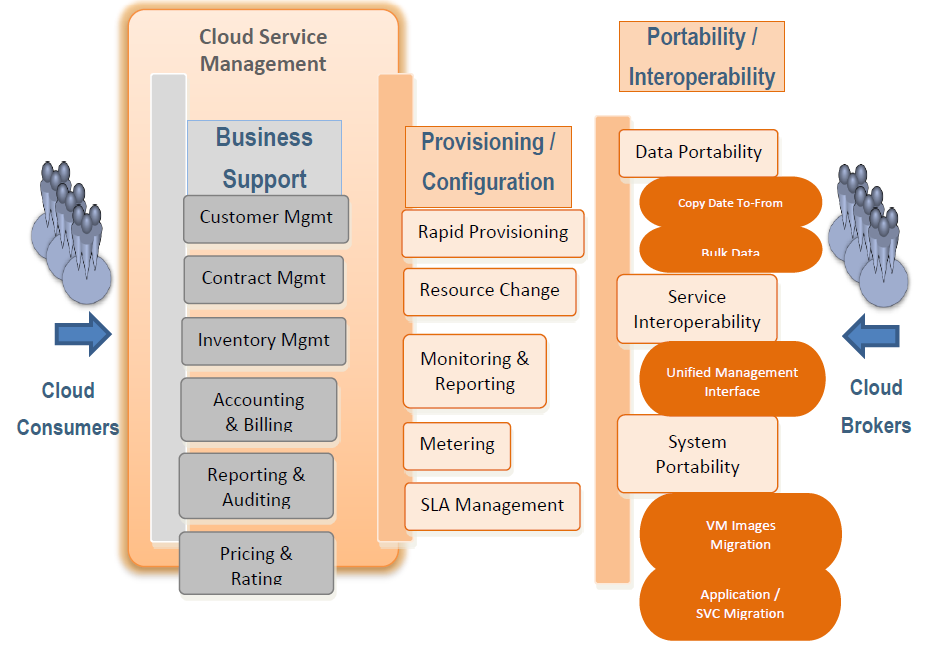
\includegraphics[width=0.8\linewidth]{images/portability}
	\caption{Portabilität in Cloudumgebungen}
	\label{fig:portability}
\end{figure*}

\subsection{OpenStack}
Unter der Bezeichnung OpenStack wird eine Plattform entwickelt, die es ermöglicht eine IaaS oder PaaS Lösung zu betreiben. Die zu OpenStack gehörigen Projekte stellen jeweils Teilaspekte des Betriebs einer Cloud Computing Lösung sicher. Die Verwaltung mehrerer virtueller Maschinen wird so z.B. durch OpenStack Compute (Nova) ermöglicht, die Verwaltung erfolgt über OpenStack Dashboard (Horizon), welches eine übersichtliche Darstellung und Konfiguration der OpenStack Plattform ermöglichen soll oder der OpenStack Database Service - Trove genannt - durch den Datenbanken als Dienst zur Verfügung gestellt werden sollen. Auch das Heat genannte Orchestrierungswerkzeug, mit dessen Hilfe Konfigurationen ("Stacks") zur automatisierten Bereitstellung und Skalierung einer ganzen Cloud-Infrastruktur realisiert werden kann, ist Teil von OpenStack.

OpenStack wurde 2010 von RackSpace Hosting zusammen mit der NASA begründet und wird mittlerweile von zahlreichen Unternehmen unterstützt, neben RackSpace zählen auch Hewlett-Packard, IBM und VMware zu den Unterstützern. Die Marktführer Amazon, Google und Microsoft zählen hingegen nicht zu den Unterstützern, die APIs der OpenStack Äquivalente zum Amazon EC2 und Amazon S3 Dienst sind jedoch kompatibel, sodass eine Portierung bestehender Anwendungen leicht möglich ist. Aufgrund der breiten Verfügbarkeit der OpenStack Ressourcen ist es möglich eigene (private) Cloud-Infrastrukturen zu erstellen und diese in die Cloud eines Cloud-Anbieters zu verschieben.

Die verschiedenen Services decken so die Bereitstellung speziell der IaaS sowie der PaaS Schicht ab.

\subsection{Docker}
Docker bietet eine Möglichkeit einen der Kritikpunkte bei der Nutzung von virtuellen Maschinen zu umgehen, indem es die Ausführung von Prozessen in vom Betriebssystem verwalteten Containern ermöglicht bzw. vereinfacht.

Während bei virtuellen Maschinen ein gesamtes Betriebssystem betrieben und von weiteren virtualisierten Instanzen getrennt wird, wird beim Einsatz von Containern nur der Prozess in einer virtualisierten Umgebung betrieben, sodass mehrere Container sich ein Hostsystem "teilen" können und dennoch voneinander getrennt auf die Ressourcen zugreifen (vergl. Abbildung \ref{fig:docker}). Die Handhabung der Container wird dabei von Linux' LXC übernommen. Überdies ermöglicht Docker auch das Erstellen und Veröffentlichen von Containern, sowie die Orchestrierung mehrerer Container einer Anwendung. Teilweise ergibt sich eine Überlappung der Möglichkeiten von OpenStack und Docker, da Docker ebenfalls in der Lage ist Images, Systemkonfigurationen oder fertige Cloudanwendungen zu erstellen und zu verwalten und es überdies z.B. auch vergleichbare Dashboard Lösungen für Docker gibt. Allerdings profitiert Docker von der Unterstützung und Verbreitung von OpenStack, da es sich gut mit OpenStack Nova integrieren lässt.

Ferner erlaubt es Docker Container über Anbietergrenzen hinweg zu verschieben und neue Anwendungsinstanzen in Containern bei unterschiedlichen Cloud-Anbietern zu starten. Die Unterstützung, vor allem durch Amazon, Google sowie Microsoft ermöglicht so tatsächliche Interoperabilität innerhalb des Cloudangebots.

\begin{figure*}
	\centering
	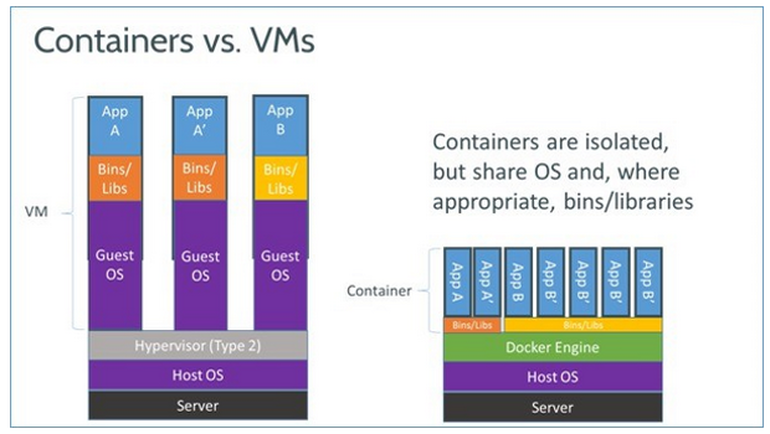
\includegraphics[width=0.8\linewidth]{images/docker-vm-container}
	\caption{Schematischer Vergleich virtuelle Maschine und Container}
	\label{fig:docker}
\end{figure*}

\section{Stand der Implementierungen}
\label{sec_implementations}
Die Cloud Computing Implementierungen in Unternehmen werden von Marktanalysten ständig überwacht und der Erfolg von Unternehmen wie Instagram, die ohne eigener Infrastruktur eine enorme Nutzerzahl erreichen konnten gibt Anlass eigene Anwendungen in die Cloud zu portieren. Dabei ergibt sich jedoch die Herausforderung, wie die zur Verfügung stehenden Möglichkeiten im Einzelfall genutzt werden können. Im allgemeinen unterscheidet sich die Herangehensweise mit Blick auf die bestehenden Systeme bzw. die Möglichkeit Neuentwicklungen zu tätigen.

\subsection{Verbreitung bei Neuentwicklungen}
Bei neuen Geschäftsmodellen oder Entwicklungen mit dem Ziel der Skalierbarkeit in Cloudumgebungen bietet sich die Nutzung von Cloudangeboten aufgrund der geringen Anschaffungskosten und Nutzungsbasierten Bezahlung an.

\subsection{Verbreitung bei bestehenden Lösungen}
Obschon Unternehmen vor allem die private Cloud nutzen möchten um die Vorzüge wie die Skaleneffekte und eine bessere Auslastung der bestehenden IT Infrastruktur zu erzielen. 

Dabei stellen jedoch bestehende Systeme eine Hürde dar, da z.B. die Infrastruktur nicht auf den Betrieb von Virtualisierungslösungen ausgelegt ist oder die bestehenden Anwendungen nicht für den Betrieb als Cloudanwendung entwickelt wurden. Speziell letzteres bedingt einen großen Portierungsaufwand oder vielmehr eine Neuentwicklung der bestehenden Anwendung. Zudem ist die Verschiebung der selbstverwalteten Lösung auf die Infrastruktur eines Cloudanbieters mit der Annahme behaftet, dass die Verfügbarkeit interner Lösungen besser sei und die Datensicherheit bei bestehenden eigenen Systemen gesichert sei.

Unter anderem aus diesen Gründen ergibt sich eine geringere Verbreitung von Cloudlösungen, wenn diese neben existierenden Systemen bestehen bzw. statt diesen eingeführt werden sollen.

\subsection{Grenzen von Cloudimplementierungen}
Aufgrund der erwünschten Skaleneffekte ist es bei private Cloud Implementierungen hilfreich die nötige Systemkapazität richtig einzuschätzen, allerdings sind Betreiber einer private Cloud häufig nicht in der Lage dies genau einzuschätzen. Aufgrund der Anzahl bestehender Hardware in großen Unternehmen wäre es für die meisten möglich ebendiese Ressourcen für den Betrieb einer private Cloud zu nutzen und die Skaleneffekte leichter zu erreichen.

Die Installation einer private Cloud stellt dabei eine größere Hürde dar, auch aufgrund der Komplexität von OpenStack  bzw. einer fehlenden direkt lauffähigen OpenStack Lösung, um eine Cloudinfrastruktur leicht aufstellen zu können. Jedoch ist auch die Elastizität der Cloudlösung in private Cloud Umgebungen limitiert, können im Bedarfsfall nicht so viele Systeme bereit gestellt werden wie sie in einer public Cloud zur Verfügung stünden.

Zudem ist die Cloud jedoch auch für kleinere Unternehmen nicht geeignet, wenn diese funktionierende bestehende Systeme betreiben und vorhersagbare Auslastungen bei diesen Systemen.